\documentclass[english]{beamer}
\usepackage[utf8]{inputenc}
\usepackage[english]{babel}
\usepackage{multicol}
\usepackage{tikz}
\usepackage{multirow}

\usepackage{subcaption}
\captionsetup{compatibility=false}

\usepackage{caption}
\captionsetup[figure]{labelformat=empty}

\usetheme[language=english,footline=sections,faculty=tw,usecolors,framenumber,totalframenumber]{UniversiteitGent}

\setbeamertemplate{caption}{\raggedright\insertcaption\par}
\setbeamertemplate{footline}
{
	\leavevmode%
	\hbox{%
		\begin{beamercolorbox}[wd=.333333\paperwidth,ht=2.25ex,dp=1ex,center]{author in head/foot}%
			\usebeamerfont{author in head/foot}\insertsection
		\end{beamercolorbox}%
		\begin{beamercolorbox}[wd=.333333\paperwidth,ht=2.25ex,dp=1ex,center]{title in head/foot}%
			\usebeamerfont{title in head/foot}\insertsubsection
		\end{beamercolorbox}%
		\begin{beamercolorbox}[wd=.333333\paperwidth,ht=2.25ex,dp=1ex,right]{date in head/foot}%
%			\usebeamerfont{date in head/foot}\insertshortdate{}\hspace*{2em}
			\insertframenumber{} / \inserttotalframenumber\hspace*{2ex} 
		\end{beamercolorbox}}%
		\vskip0pt%
	}

\usetikzlibrary{arrows}
\usetikzlibrary{fit}
\usetikzlibrary{calc}
\usetikzlibrary{backgrounds}
\usetikzlibrary{shapes.geometric}
\usetikzlibrary{positioning}

\tikzset{hide on/.code={\only<#1>{\color{white}}}}
\tikzset{
	invisible/.style={opacity=0},
	visible on/.style={alt=#1{}{invisible}},
	alt/.code args={<#1>#2#3}{%
		\alt<#1>{\pgfkeysalso{#2}}{\pgfkeysalso{#3}} % \pgfkeysalso doesn't change the path
	},
	level/.style={sibling distance = 4cm/#1,level distance = 1.5cm},
	treenode/.style = {align=center, inner sep=0pt, text centered,
		font=\ttfamily},
	arn_l/.style = {treenode, circle, ugentblue, draw=ugentblue, fill=ugentyellow,
		text width=1.5em, very thick},% leaf node
	arn_x/.style = {treenode, circle, white, draw=ugentblue, fill=ugent-pp,
		text width=1.5em, very thick},% red
	arn_y/.style = {treenode, circle, white, draw=ugentblue, fill=ugent-tw,
		text width=1.5em, very thick},% blue
	arn_0/.style = {treenode, draw=none,
		fill=none, text width=0},% hidden node
	arn_s/.style = {treenode, circle,
		fill=ugentblue, text width=0.75em},%small node
	rect_l/.style ={shape=rectangle, rounded corners, draw, align=center,
		color=ugentblue, top color=ugentyellow, bottom color=ugentyellow, very thick},
	rect_x/.style ={shape=rectangle, rounded corners, draw, align=center,
		color=ugentblue, top color=ugent-pp, bottom color=ugent-pp, very thick},
}


\AtBeginSection[]
{
	\begin{frame}
		\begin{columns}[t]
			\begin{column}{5cm}
				\tableofcontents[sections={1-4},currentsection, hideothersubsections]
			\end{column}
			\begin{column}{5cm}
				\tableofcontents[sections={5-8},currentsection,hideothersubsections]
			\end{column}
		\end{columns}
	\end{frame}
}


\title{Design of a diagnosis and follow-up platform for patients with chronic headaches}
%\subtitle{Phylogeny Comparison}
\author{Kiani Lannoye \& Gilles Vandewiele}
\mode<beamer>{\institute{Faculty of Engineering and Architecture}}

\begin{document}
\begin{frame}
	\titlepage
\end{frame}

\begin{frame}
	\begin{columns}[t]
		\begin{column}{5cm}
			\tableofcontents[sections={1-4},currentsection, hideothersubsections]
		\end{column}
		\begin{column}{5cm}
			\tableofcontents[sections={5-8},currentsection,hideothersubsections]
		\end{column}
	\end{columns}
\end{frame}

\section{Intro}
\label{sec:intro}
\begin{frame}{Introduction}
	\framesubtitle{test}
	\begin{figure}[!h]
		\centering
		
\includegraphics[width=\textwidth]{figures/headache.jpg}
	\end{figure}
\end{frame}

\begin{frame}{Headaches}
	\begin{figure}[!h]
		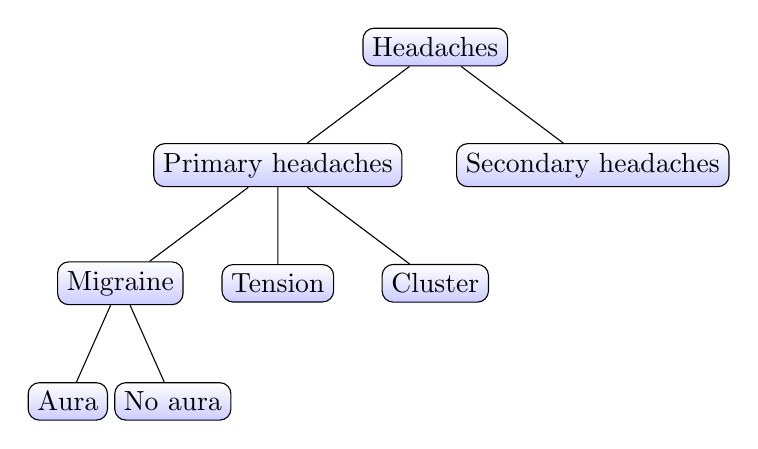
\begin{tikzpicture}[sibling distance=10em,
		every node/.style = {shape=rectangle, rounded corners,
			draw, align=center,
			top color=white, bottom color=blue!20}]]
		\only<5>{}
		\node {Headaches}
		child[visible on=<2->] { 
			node {Primary headaches} 
				child[visible on=<4->] {
					node {Migraine}
						child[visible on=<5->] {
							node {Aura}
						}
						child[visible on=<5->]{
							node {No aura}
						}
				}
				child[visible on=<4->] {
					node {Tension}
				}
				child[visible on=<4->] {
					node {Cluster}
				}
		}
		child[visible on=<3->] { node {Secondary headaches}};
		\end{tikzpicture}
	\end{figure}
\end{frame}
\subsection{Current process UH Ghent}

\begin{frame}{Current process UH Ghent}
	Current process at UH Ghent is:
	\begin{itemize}
		\item Not digital
		\item cumbersome
		\item long-lasting
	\end{itemize}
\end{frame}

\begin{frame}
	\framesubtitle{Current process at UH Ghent}
	\begin{figure}[!h]
		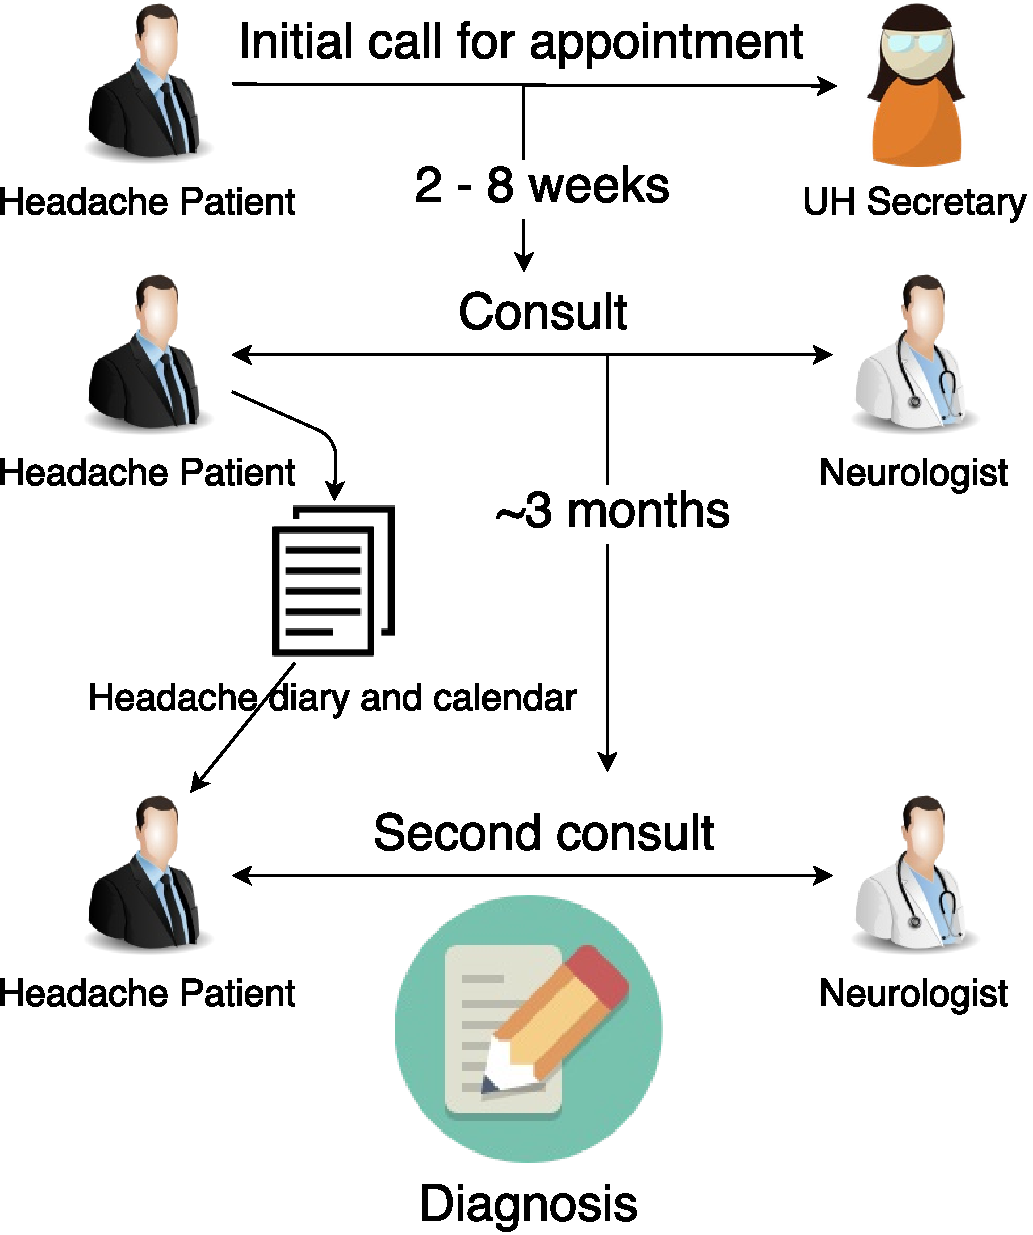
\includegraphics[width=0.5\textwidth]{figures/UZ_patient.pdf}
	\end{figure}
\end{frame}

\begin{frame}
	So there is need for a better (digital) alternative! This alternative has to:
	\begin{itemize}
		\item capture at least the same information as current solution
		\item be more efficient
		\item provide a second opinion for the doctors (auto-diagnose)
	\end{itemize}
\end{frame}
% section intro (end)
\section{Platform requirements}
\label{sec:platform_req}
\begin{frame}
	\frametitle{Platform requirements}


		Our proposed alternative consists of:
		\begin{itemize}
			\item Headache journal: mobile app
			\item Doctor Dashboard: web application
			\item Machine learning module: auto-classify
		\end{itemize}
		\ \newline
		Solution non-functional requirements:
		\begin{itemize}
			\item Security
			\item Availability
			\item Performance
			\item Usability
		\end{itemize}
\end{frame}
\begin{frame}
		\frametitle{Platform requirements}
		\begin{figure}[!h]
			\includegraphics[width=\textwidth]{figures/system_analysis.png}
		\end{figure}	
	
\end{frame}
% section Platform requirements (end)
\section{Mobile application}
\begin{frame}{Mobile Application}
	Why create a new application? 
	\begin{block}{Competition}{}
		\begin{itemize}
			\item Migraine Buddy
			\item Headache Diary
			\item Pfizer headache journal
		\end{itemize}
	\end{block}
	\pause
	All good, but:
	\pause
	\begin{itemize}
		\item none offers usable data export
		\item none captures all data needed
	\end{itemize} 
\end{frame}
\subsection{Development paradigms}
\begin{frame}{Development paradigms}
	Different kinds of approaches for mobile application development:
	\begin{itemize}
		\item Web application
		\item Hybrid application
		\item Native application
	\end{itemize}
	$\rightarrow$ How do we choose?
\end{frame}
\begin{frame}{Web application}
	Webapps are developed once and can be viewed on (almost) all smartphones (via built-in web engine).\newline
	\newline
	$+$ ``write once, run everywhere'' $\Rightarrow$ lower cost\newline
	$+$ No installation required\newline
	$-$ limited use of device specific features (GPS, camera, ...)\newline
	\textbf{$-$ Not all devices same web engines $\Rightarrow$ other view}\newline
	$-$ No native look and feel\newline
	\newline
	{\Large \color{red}  $\Rightarrow$ No web application}
\end{frame}

\begin{frame}{Native application}
	Native apps are developed once for each OS and installed on the device.\newline
	\newline
	$+$ Best performance (optimized machine code at compile time)\newline
	$+$ Device specific features usable (GPS, camera, ...)\newline
	$+$ Native look and feel\newline
	\textbf{$-$ Write code for each OS (very costly dev + maintenance)}\newline
	$-$ Installation required\newline
	\newline
	{\Large \color{red}  $\Rightarrow$ Native application?}
\end{frame}

\begin{frame}{Hybrid application}
	Hybrid apps are developed once and installed on the device. It uses the devices internal web engine, but has more control than web applications.\newline
	\newline
	$+$ ``write once, run everywhere'' $\Rightarrow$ lower cost\newline
	$+$ Better performance (semi-optimized machine code)\newline
	$+$ Device specific features usable (GPS, camera, ...)\newline
	$+$ Native look and feel (using libraries)\newline
	$-$ Installation required\newline
	\textbf{$-$ Not all devices same web engines $\Rightarrow$ other view\newline (but manageable)}
		\vspace{0.8em}

	{\Large \color{red}  $\Rightarrow$ Hybrid application?}
\end{frame}

\begin{frame}{Hybrid vs Native}
	\only<2>{}
\begin{tabular}{l||ll}
	& \textbf{\color<2>{red}Native}                                                                                                                          & \textbf{\color<2>{green}Cross-platform}                                                                                                                                                                            \\ \hline \hline
	\textbf{+}    & \begin{tabular}[c]{@{}l@{}}+ Native UX\\ + device-specific features\\ + Better performance\end{tabular}               & \begin{tabular}[c]{@{}l@{}}+ 1 language\\ + Write once, run everywhere\\ + Less maintenance\end{tabular}                                                                \\ \hline
	\textbf{-} & \begin{tabular}[c]{@{}l@{}}- Multiple languages\\ - Time consuming \\ \ (development)\end{tabular} & \begin{tabular}[c]{@{}l@{}}- Slower (lower performance)\\ - Less device specific\\ \hspace{0.4em}  features\\ - Harder to release online\\ \hspace{0.4em} (Play Store/App Store)\end{tabular}
\end{tabular}
\end{frame}
\subsection{Chronicals}
\begin{frame}
				\centering
	\only<1>{\begin{tabular}{c}
			\centering
			\includegraphics[height=0.7\paperheight]{figures/chronicals.png}
		\end{tabular}}
	\only<2>{	
	 \begin{tabular}{cl}  
	 	\begin{tabular}{c}
			\includegraphics[height=0.7\paperheight]{figures/chronicals.png}
	 	\end{tabular}
	 	& \begin{tabular}{l}
			 \parbox{0.4\linewidth}{
			 	\centering
				{\Huge{Chronicals}\newline}
				\newline
				
\includegraphics[height=0.3\paperheight]{figures/QR_code.png}
			}
	 	\end{tabular}  \\
	 \end{tabular}
	}
\end{frame}
\begin{frame}{Chronicals}
\begin{figure}[!h]
	\centering
	\begin{subfigure}[b]{0.3\textwidth}
		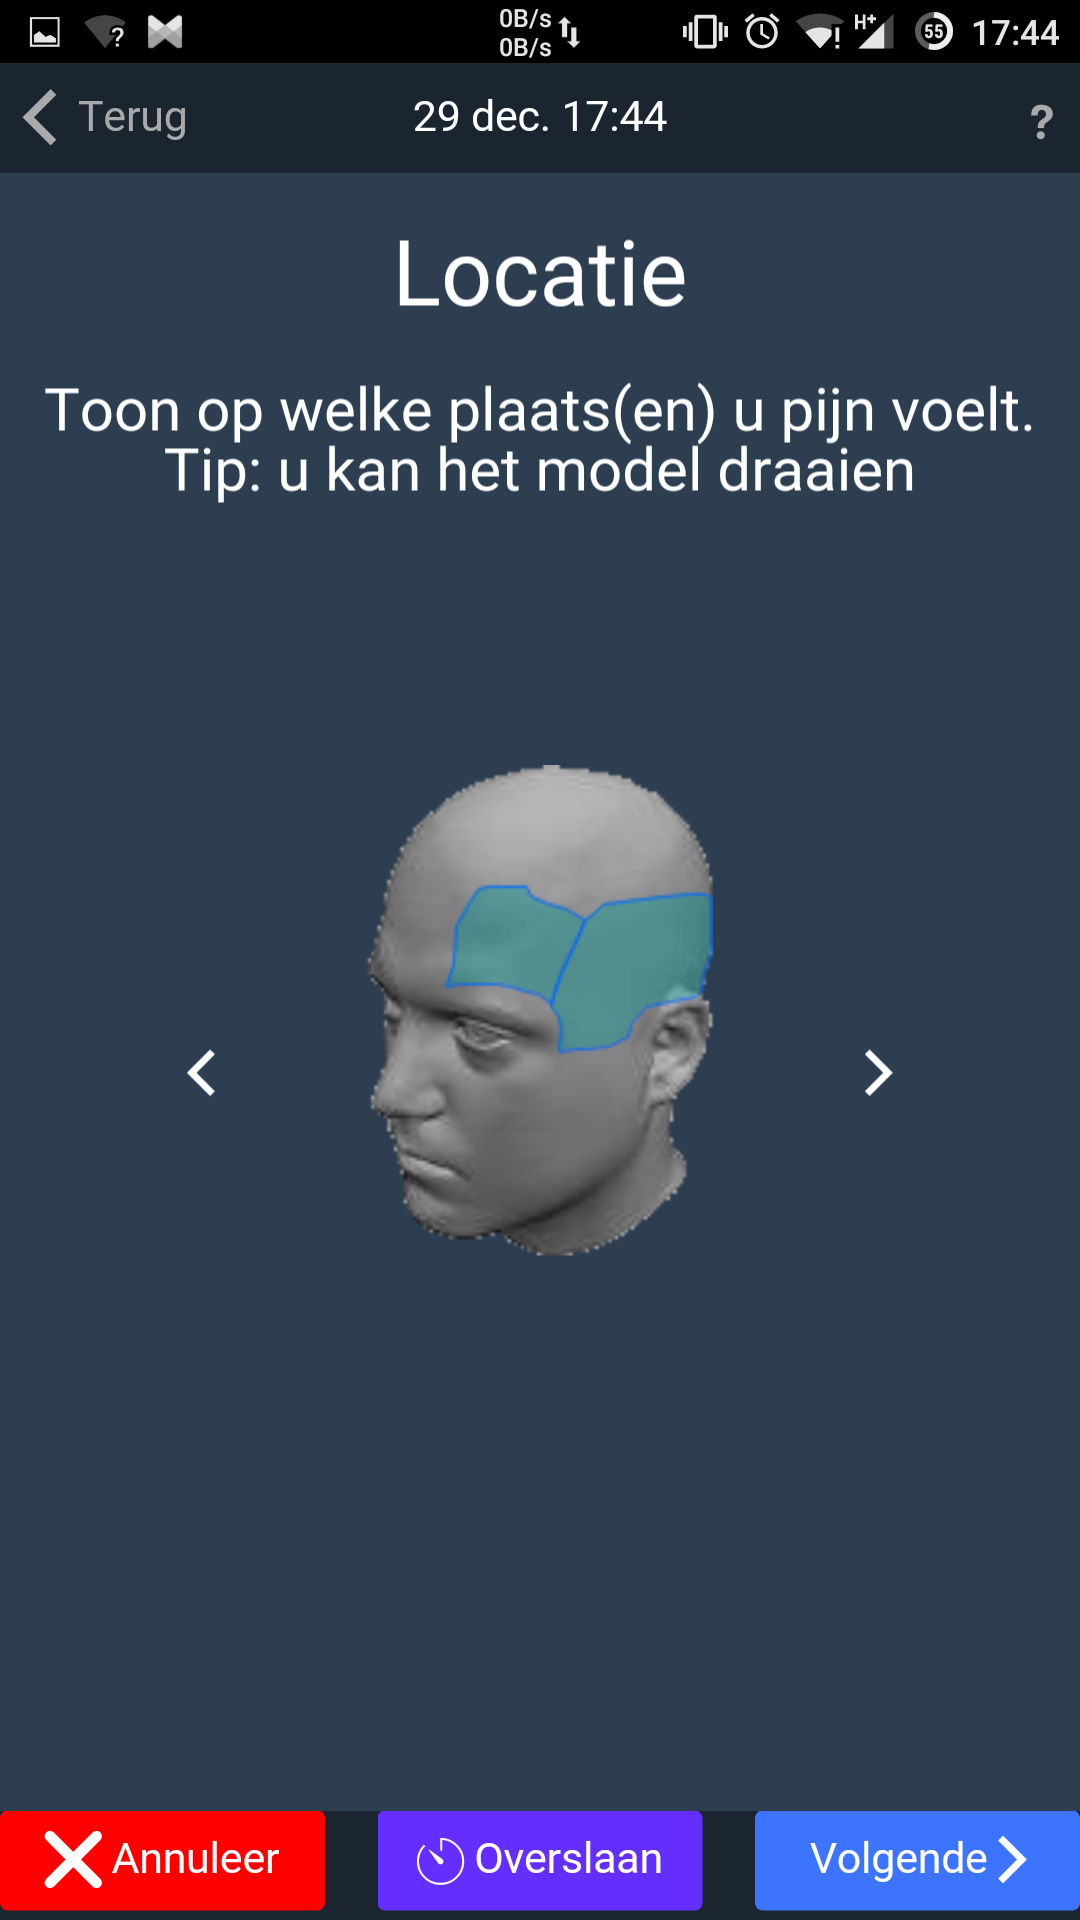
\includegraphics[width=\textwidth]{figures/add_headache_5.png}
	\end{subfigure}
	\pause
	~ %add desired spacing between images, e. g. ~, \quad, \qquad, \hfill etc. 
	%(or a blank line to force the subfigure onto a new line)
	\begin{subfigure}[b]{0.3\textwidth}
		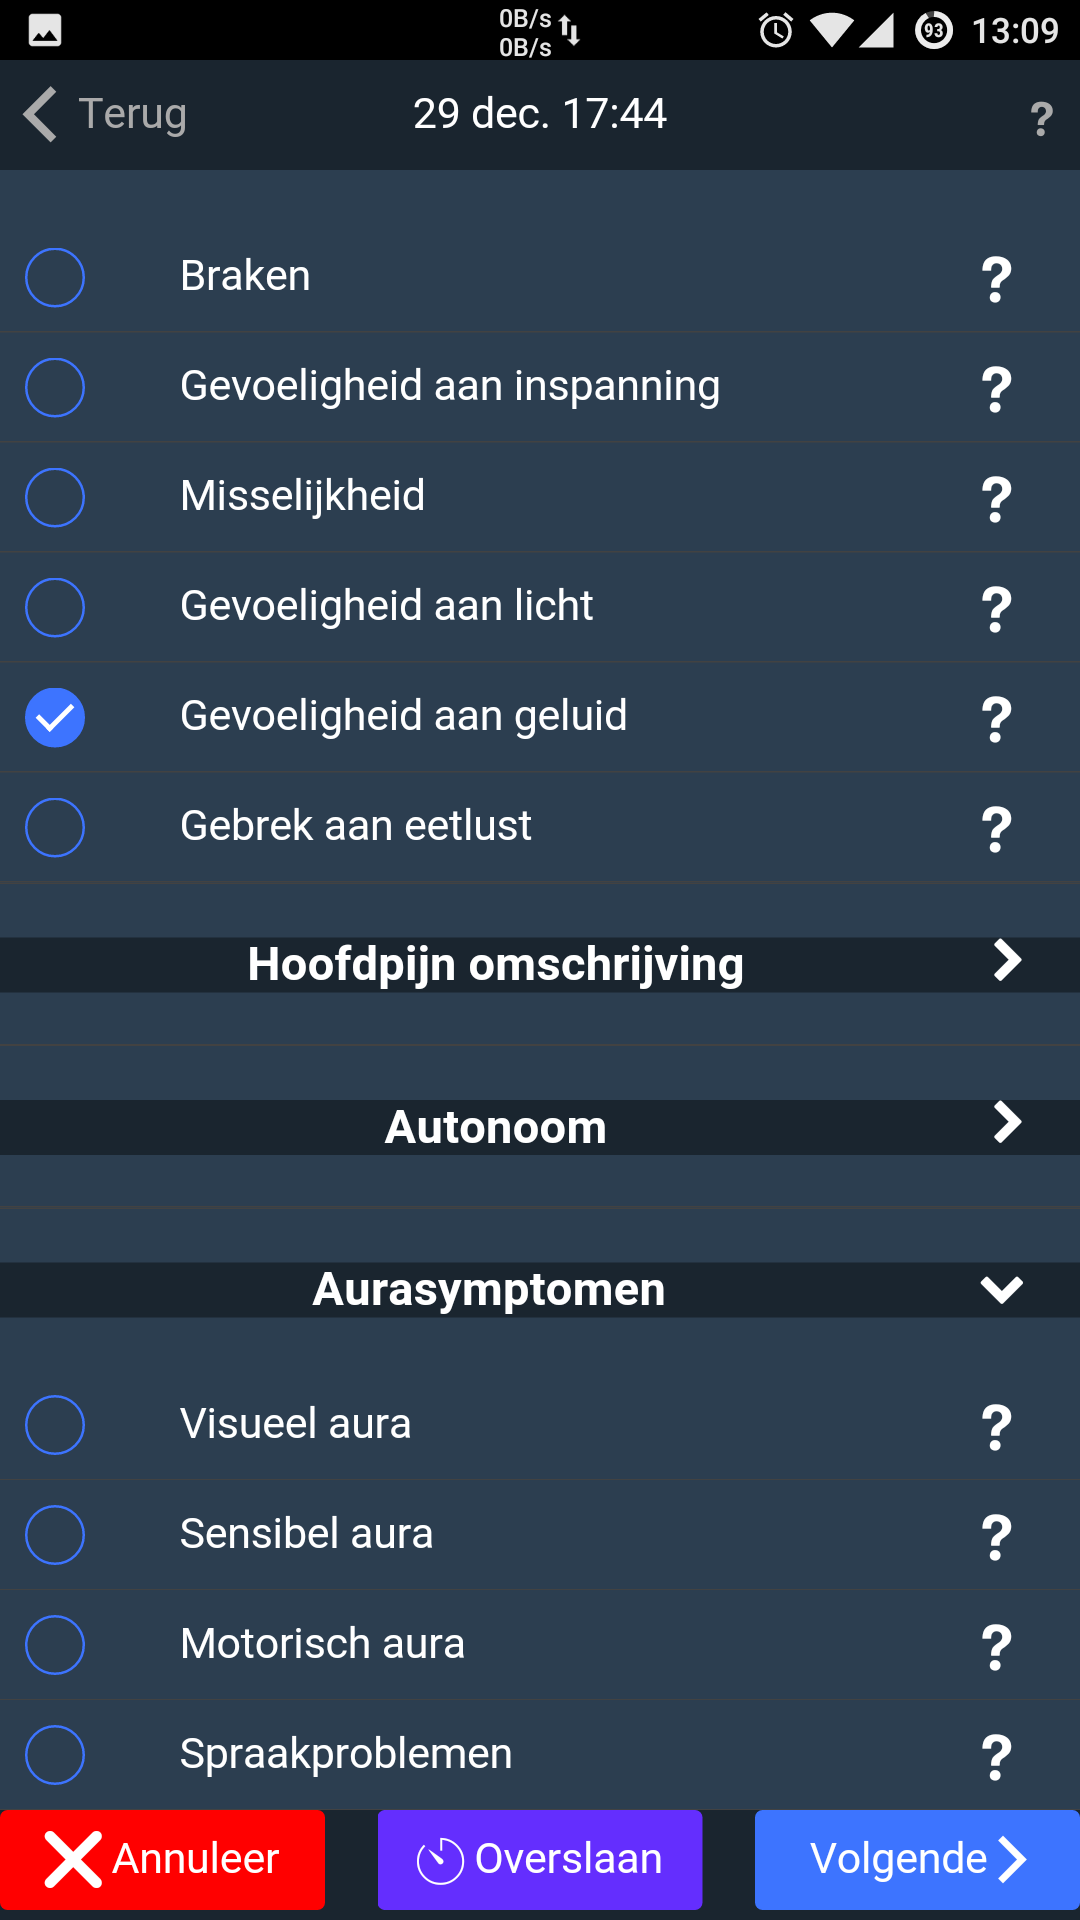
\includegraphics[width=\textwidth]{figures/add_headache_6.png}
	\end{subfigure}
	\pause
	~ %add desired spacing between images, e. g. ~, \quad, \qquad, \hfill etc. 
	%(or a blank line to force the subfigure onto a new line)
	\begin{subfigure}[b]{0.3\textwidth}
		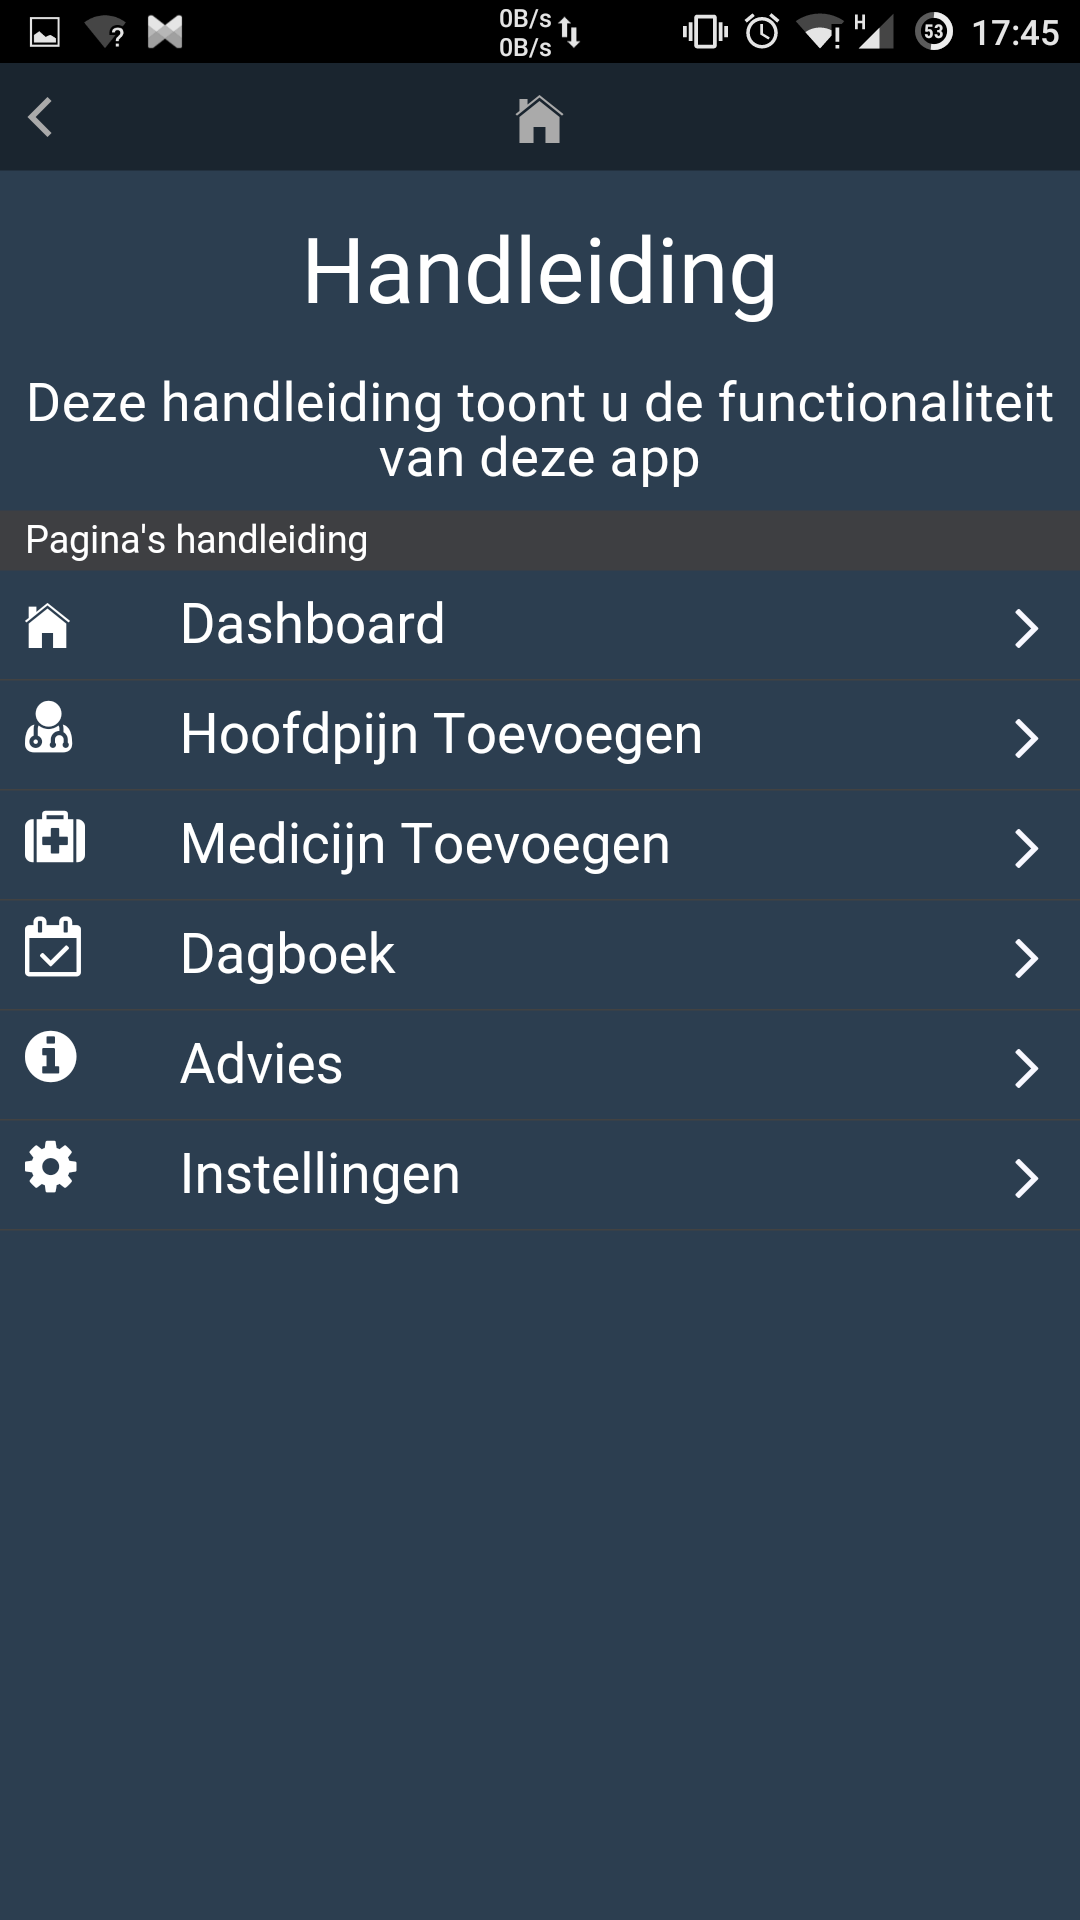
\includegraphics[width=\textwidth]{figures/manual.png}
	\end{subfigure}
\end{figure}
\end{frame}
\section{Backend and data exposure}
\begin{frame}{Backend and data exposure}
	\begin{block}{Components}
		\begin{itemize}
			\item Database
			\item Connection to App
			\item Connection to Docter Dashboard
			\item Connection Machine learning module
		\end{itemize}
	\end{block}
\end{frame}
\begin{frame}{System}
	\begin{figure}[!h]
		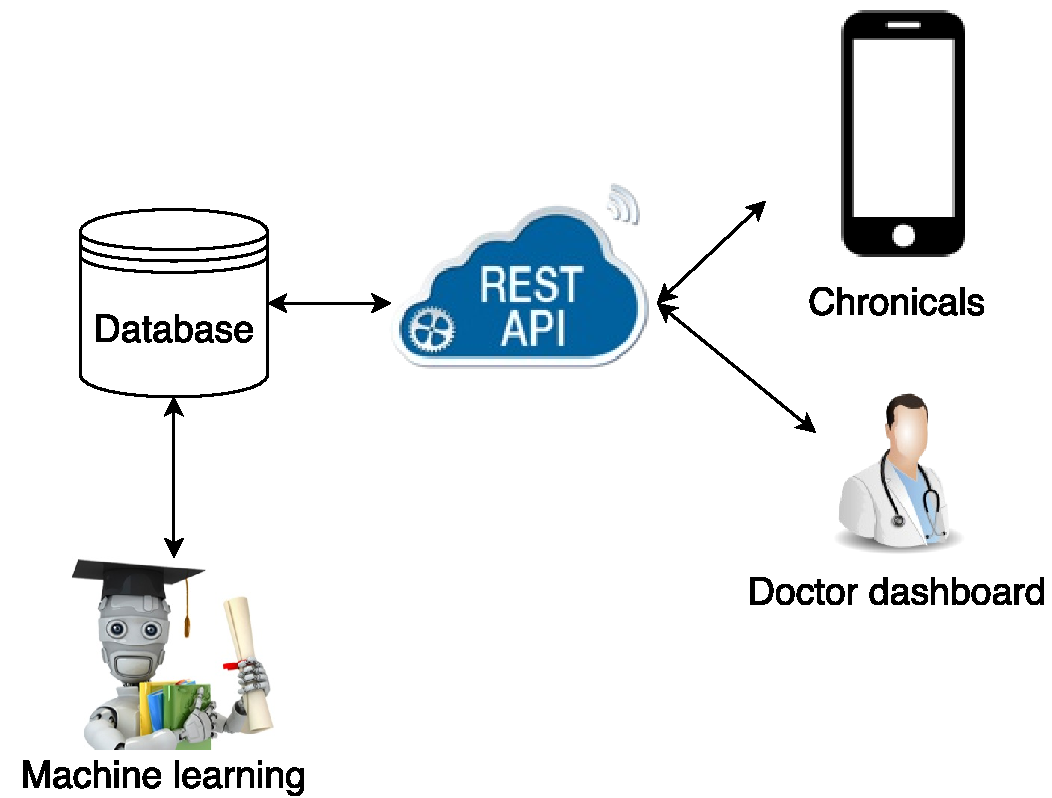
\includegraphics[width=0.6\textwidth]{figures/Data exposure.pdf}
	\end{figure}	
\end{frame}
\section{Machine learning - DT's}

\subsection*{Why decision trees?}

\subsection*{Decision tree induction algorithms}

\subsection*{Ensemble techniques}

\section{Genetic merging of DT's}
\subsection*{Introduction}

\begin{frame}{Many different induction algorithms}
	\begin{columns}
		\begin{column}{0.25\textwidth}
			\centering
			\begin{figure}
				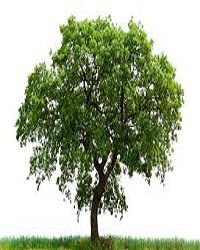
\includegraphics[width=\textwidth]{figures/oak.jpg}
				\caption{C4.5 (C5.0)}
			\end{figure}
		\end{column}
		\begin{column}{0.25\textwidth}
			\centering
			\begin{figure}
				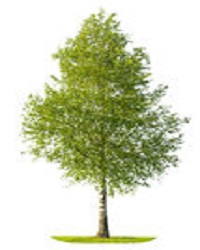
\includegraphics[width=\textwidth]{figures/berk.jpg}
				\caption{CART}
			\end{figure}
		\end{column}
		\begin{column}{0.25\textwidth}
			\centering
			\begin{figure}
				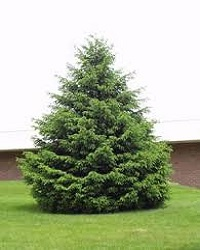
\includegraphics[width=\textwidth]{figures/spar.jpg}
				\caption{QUEST}
			\end{figure}
		\end{column}
		\begin{column}{0.25\textwidth}
			\centering
			$\ldots$
		\end{column}
	\end{columns}
	
	\textbf{$\rightarrow$ Which tree is the most beautiful?}
\end{frame}

\begin{frame}{Current ensembles lack interpretability}
	\begin{block}{}
	\textbf{Boosting, bagging, random forests,} etc. require majority voting (classification) or mean calculation (regression) to obtain prediction
	\end{block}
	
	\vspace{3em}
	\resizebox{0.24\textwidth}{!}{%
	\begin{tikzpicture}
	\node (A) [arn_l] {};
	\node (B) [arn_l, below left=0.75cm and 0.75 cm of A] {};
	\node (C) [arn_l, below right=0.75cm and 0.75 cm of A] {};
	\node (D) [rect_l, below left of=B] {0};
	\node (E) [rect_l, below right of=B] {1};
	\node (F) [rect_l, below left of=C] {1};
	\node (G) [rect_x, below right of=C] {0};
	\draw (A) -- (B);
	\draw (A) -- (C);
	\draw (B) -- (D);
	\draw (B) -- (E);
	\draw (C) -- (F);
	\draw (C) -- (G);
	\end{tikzpicture}%
	 } \resizebox{0.24\textwidth}{!}{%
		\begin{tikzpicture}
		\node (A) [arn_l] {};
		\node (B) [arn_l, below left=0.75cm and 0.75 cm of A] {};
		\node (C) [arn_l, below right=0.75cm and 0.75 cm of A] {};
		\node (D) [rect_l, below left of=B] {0};
		\node (E) [rect_l, below right of=B] {1};
		\node (F) [rect_l, below left of=C] {1};
		\node (G) [rect_x, below right of=C] {0};
		\draw (A) -- (B);
		\draw (A) -- (C);
		\draw (B) -- (D);
		\draw (B) -- (E);
		\draw (C) -- (F);
		\draw (C) -- (G);
		\end{tikzpicture}%
		 } \resizebox{0.24\textwidth}{!}{ %		
	 	$\ldots$ %
		}	\resizebox{0.24\textwidth}{!}{%
		\begin{tikzpicture}
		\node (A) [arn_l] {};
		\node (B) [arn_l, below left=0.75cm and 0.75 cm of A] {};
		\node (C) [arn_l, below right=0.75cm and 0.75 cm of A] {};
		\node (D) [rect_l, below left of=B] {0};
		\node (E) [rect_x, below right of=B] {1};
		\node (F) [rect_l, below left of=C] {1};
		\node (G) [rect_l, below right of=C] {0};
		\draw (A) -- (B);
		\draw (A) -- (C);
		\draw (B) -- (D);
		\draw (B) -- (E);
		\draw (C) -- (F);
		\draw (C) -- (G);
		\end{tikzpicture}%
		 }
	
	\framesubtitle{Stacking}
\end{frame}

\begin{frame}{Current ensembles lack interpretability}
	\begin{block}{}
		The final decision tree obtained by \textbf{stacking} contains uninterpretable internal nodes
	\end{block}
	
	\vspace{2em}
	
	\begin{tikzpicture}
	\centering
	\node (A) [rect_l] {$x_1 \leq 5.0$};
	\node (B) [rect_x, below left=0.75cm and 0.75 cm of A] {$outcome_{NN} \leq 2.0$};
	\node (C) [rect_x, below right=0.75cm and 0.75 cm of A] {$outcome_{RF} \leq 4.0$};
	\node (D) [rect_l, below left=0.5cm and 0.5cm of B] {0};
	\node (E) [rect_l, below right=0.5cm and 0.5cm of B] {1};
	\node (F) [rect_l, below left=0.5cm and 0.5cm of C] {0};
	\node (G) [rect_l, below right=0.5cm and 0.5cm of C] {1};
	\draw (A) -- (B);
	\draw (A) -- (C);
	\draw (B) -- (D);
	\draw (B) -- (E);
	\draw (C) -- (F);
	\draw (C) -- (G);
	\end{tikzpicture}
	
\end{frame}

\subsection*{Merging different DT's}

\begin{frame}{Decision tree $\rightarrow$ decision space}
	\begin{block}{Converting decision trees to decision spaces}
		We can define a one-to-one mapping between a decision tree and a set of $k$-dimensional hyperplanes ($k$ = $\#$features), called \textbf{decision~space}.	Each node in the decision tree corresponds to a hyperplane in the decision space.
	\end{block}
\end{frame}

\begin{frame}{Decision tree $\rightarrow$ decision space}
	\begin{figure}
		\centering
		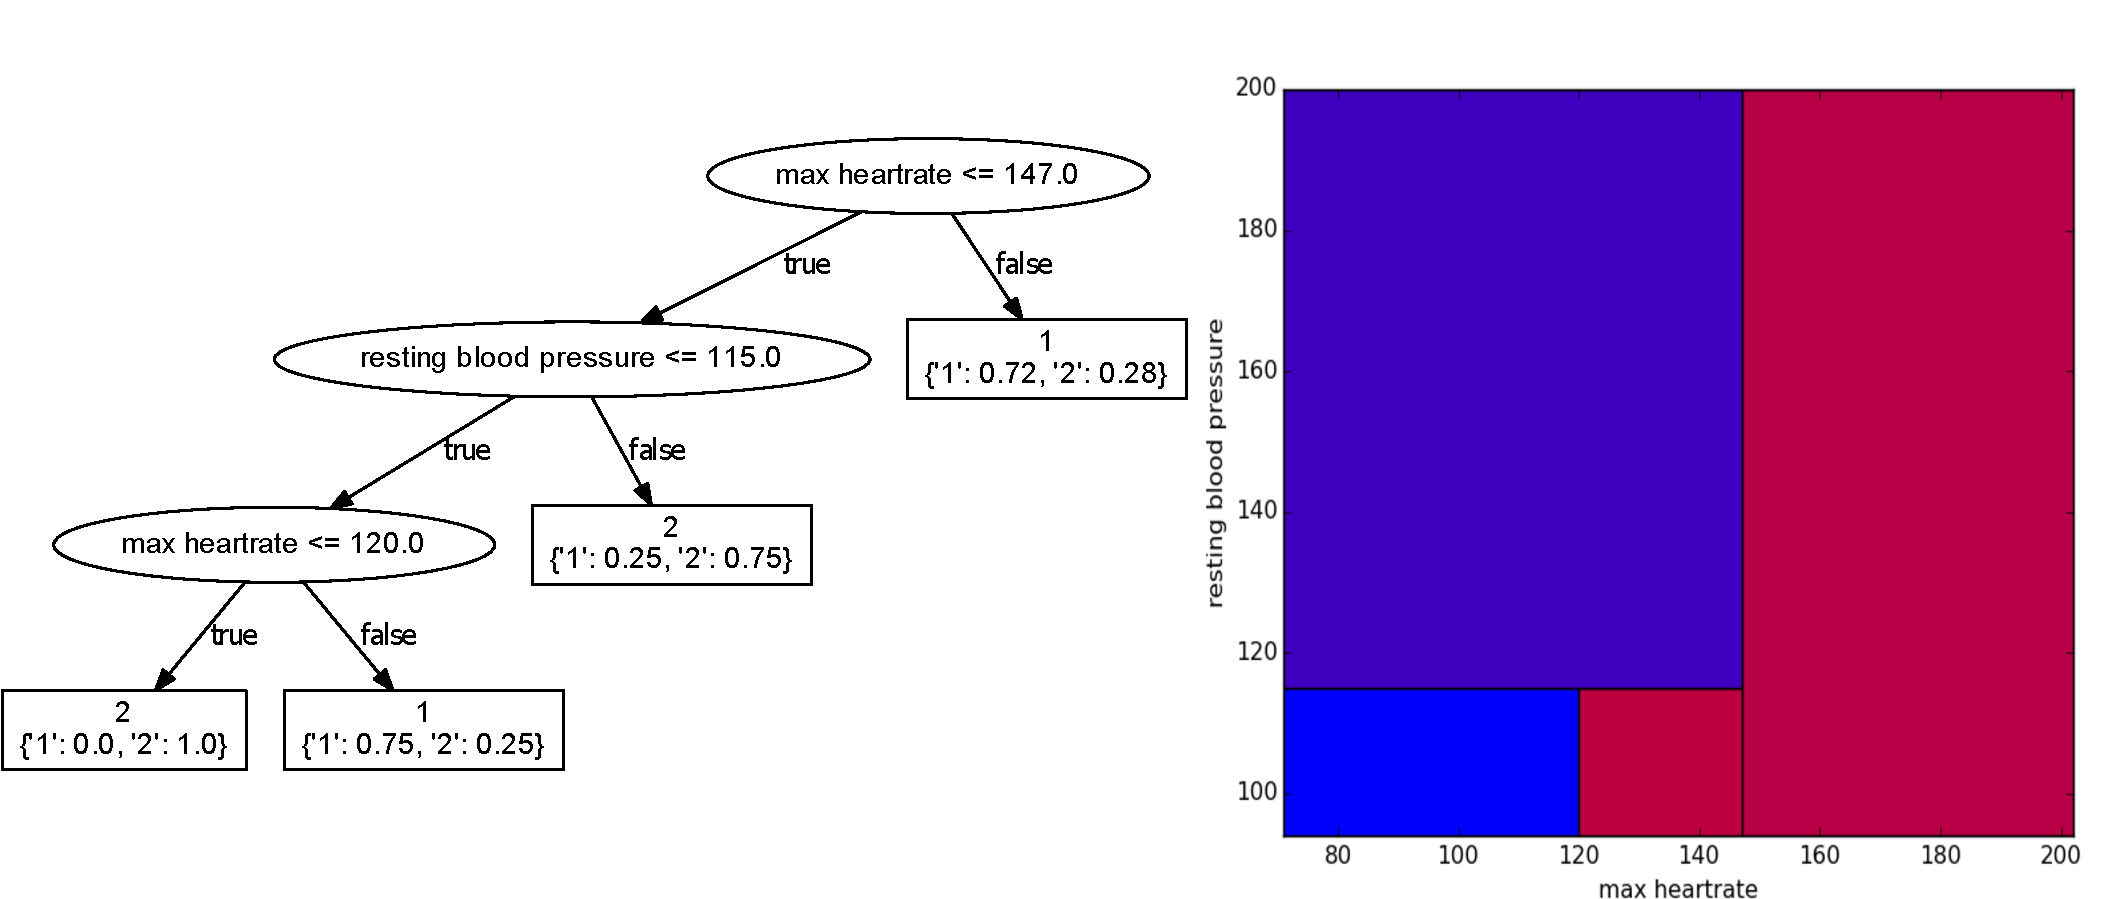
\includegraphics[width=\textwidth]{figures/dt_to_space.pdf}
	\end{figure}
\end{frame}

\begin{frame}{Merging decision spaces}
	\begin{figure}
		\centering
		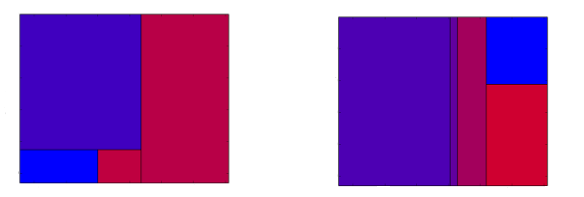
\includegraphics[width=\textwidth]{figures/merge_space_1.png}
	\end{figure}
\end{frame}

\begin{frame}{Merging decision spaces}
	\begin{figure}
		\centering
		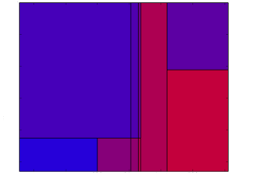
\includegraphics[scale=1]{figures/merge_space_2.png}
	\end{figure}
\end{frame}

\begin{frame}{Pruning decision spaces}
	\begin{figure}
		\centering
		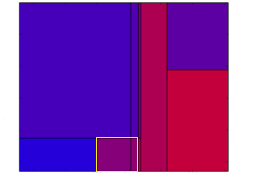
\includegraphics[scale=1]{figures/pruning.png}
	\end{figure}
\end{frame}

\begin{frame}{Decision space $\rightarrow$ decision tree}
	\begin{block}{Converting decision spaces to decision trees}
		One-to-one mapping from decision tree to space is lost during conversion because the order is lost. Therefore, a heuristic approach must be taken, identifying hyperplane candidates and calculating a metric to choose the `best' plane.
	\end{block}
	
	
	\begin{block}{Candidate hyperplanes}
		In order for a plane to be the next candidate node, it must be unbounded in all dimensions but one.
	\end{block}
\end{frame}

\begin{frame}{Decision space $\rightarrow$ decision tree}
	\begin{figure}
		\centering
		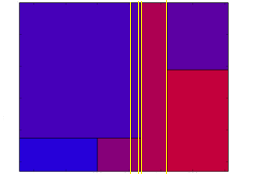
\includegraphics[scale=1]{figures/space_to_dt.png}
	\end{figure}	
\end{frame}

\begin{frame}{Decision space $\rightarrow$ decision tree}
	\begin{block}{Finding `best' candidate hyperplane}
		Apply metric function to each plane, these include:
		\begin{itemize}
			\item information gain and Gini from C4.5 and CART respectively
			\item pick plane from most correlated feature ($\chi^2$- and ANOVA $F$-test from QUEST)
			\item pick plane that divide space in two most equal subspaces (using surface/volume or counting number of planes)
			\item combination
		\end{itemize}
	\end{block}
	
\end{frame}


\subsection*{Genetic algorithm}
{\setbeamertemplate{footline}{}
\begin{frame}{}
	\begin{figure}
		\centering
		\includegraphics[scale=0.33]{figures/genetic.png}
	\end{figure}	
\end{frame} }

\begin{frame}{Splitting the data}
	\vspace{-1em}
	\begin{figure}
		\centering
		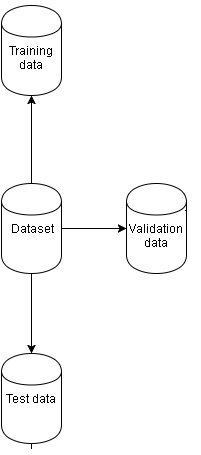
\includegraphics[scale=0.5]{figures/split_data.png}
	\end{figure}	
\end{frame}

\begin{frame}{Generate different decision trees}
	\vspace{-2em}
	\begin{figure}
		\centering
		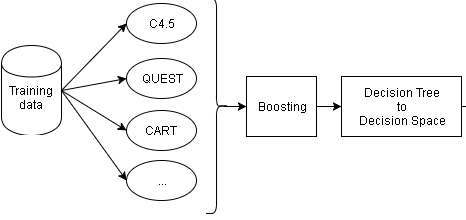
\includegraphics[scale=0.8]{figures/generate_dt.png}
	\end{figure}	
\end{frame}

\begin{frame}{Generate different decision trees}
	\begin{figure}
		\centering
		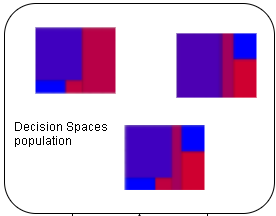
\includegraphics[scale=1]{figures/dt_population.png}
	\end{figure}	
\end{frame}

{\setbeamertemplate{footline}{}
\begin{frame}{Genetic merging}
	\begin{figure}
		\centering
		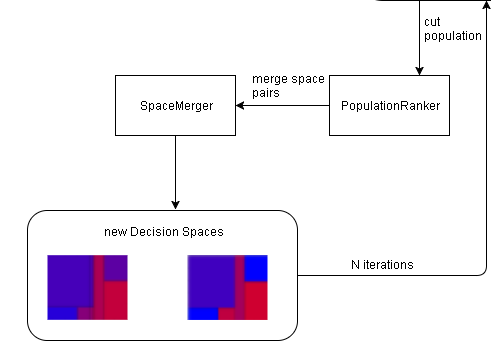
\includegraphics[scale=0.7]{figures/genetic_merging.png}
	\end{figure}
\end{frame} }

{\setbeamertemplate{footline}{}
\begin{frame}{Final iteration}
	\vspace{-1em}
	\begin{figure}
		\centering
		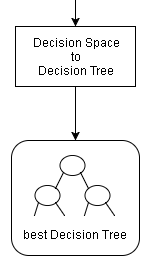
\includegraphics[scale=0.7]{figures/final_iteration.png}
	\end{figure}
\end{frame} }



\begin{frame}{Evaluating our algorithm}
	\begin{block}{}
		To test how good our algorithm performs, we downloaded 5 datasets from the UCI machine learning repository. We then compared our genetic merging algorithm with the three discussed decision tree induction algorithms, using optimal parameters, feature selection when needed and k-fold cross-validation.
	\end{block}
\end{frame}

\begin{frame}{Heart disease dataset}
	\begin{columns}
		\begin{column}{0.35\textwidth}
			\begin{figure}
				\centering
				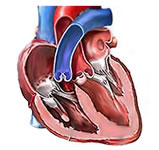
\includegraphics[scale=0.75]{figures/heart.jpg}
			\end{figure}
		\end{column}
		
		\begin{column}{0.65\textwidth}
			\begin{itemize}
				\item medical dataset
				\item 270 samples
				\item 13 features: 6 continuous (max heartrate), 7 discrete (sex)
				\item 2 classes: sick or healthy
				\item more healthy than sick samples
				\item false negatives can cost lives!
			\end{itemize}
		\end{column}
	\end{columns}
\end{frame}

\begin{frame}{Car evaluation dataset}
	\begin{columns}
		\begin{column}{0.35\textwidth}
			\begin{figure}
				\centering
				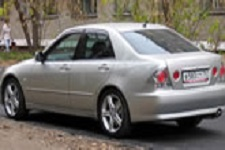
\includegraphics[scale=1]{figures/car.jpg}
			\end{figure}
		\end{column}
		
		\begin{column}{0.65\textwidth}
			\begin{itemize}
				\item 1725 samples
				\item only 6 features, all categories (price, doors, $\ldots$)
				\item 4 classes: unacceptable, acceptable, good and very good
				\item VERY imbalanced (70\% unacc, 22.2\% acc)
			\end{itemize}
		\end{column}
	\end{columns}
\end{frame}

\begin{frame}{Iris flowers dataset}
	\begin{columns}
		\begin{column}{0.35\textwidth}
			\begin{figure}
				\centering
				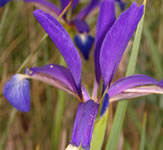
\includegraphics[scale=0.75]{figures/iris.jpg}
			\end{figure}
		\end{column}
		
		\begin{column}{0.65\textwidth}
			\begin{itemize}
				\item very small dimensions
				\item 150 flowers
				\item 4 continuous features (petal width and sepal length)
				\item 3 classes: setosa, versicolor, virginica
				\item perfectly balanced (50-50-50)
			\end{itemize}
		\end{column}
	\end{columns}
\end{frame}

\begin{frame}{Shuttle classification dataset}
	\begin{columns}
		\begin{column}{0.35\textwidth}
			\begin{figure}
				\centering
				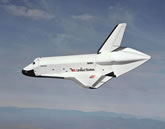
\includegraphics[scale=0.75]{figures/shuttle.jpg}
			\end{figure}
		\end{column}
		
		\begin{column}{0.65\textwidth}
			\begin{itemize}
				\item originally: 58000 samples corresponding to aircrafts
				\item here: 14500 samples
				\item 9 numerical attributes
				\item 7 different types of shuttles: 2 of them contained less than 10 samples (discarded)
			\end{itemize}
		\end{column}
	\end{columns}
\end{frame}

\begin{frame}{Nursery application dataset}
	\begin{columns}
		\begin{column}{0.35\textwidth}
			\begin{figure}
				\centering
				
\includegraphics[scale=0.75]{figures/nursery.jpg}
			\end{figure}
		\end{column}
		
		\begin{column}{0.65\textwidth}
			\begin{itemize}
				\item 12960 samples (applications for nursery school)
				\item 8 categorical features
				\item 5 classes: not recommended, recommended, very recommended, priority and special priority
				\item only 2 samples were recommended (discarded)
			\end{itemize}
		\end{column}
	\end{columns}
\end{frame}

\begin{frame}{}
	\vspace{-1em}
	\begin{table}
		\begin{tabular}{|c|c|c|c|c|c|}
			\hline \textbf{Dataset} & \textbf{Folds} & \textbf{C4.5} & \textbf{CART} & \textbf{QUEST} & \textbf{Genetic} \\ \hline
			\multirow{2}{*}{Heart disease} & 5 & $\textbf{0.8067}$ & $0.7844$ & $0.7844$ & $\textbf{0.8067}$ \\
			& 10 & $\textbf{0.8104}$ & $0.7732$ & $0.7881$ & $0.7993$ \\ \hline
			\multirow{2}{*}{Iris} & 3 & $0.9533$ & $0.9467$ & $0.9467$ & $\textbf{0.96}$ \\ & 5 & $0.9467$ & $0.9333$ & $0.9467$ & $\textbf{0.9533}$ \\ \hline
			\multirow{3}{*}{Cars} & 3 & $\textbf{0.9722}$ & $0.9693$ & $0.9229$ & $0.9693$ \\
			& 5 & $0.9711$ & $0.9682$ & $0.9241$ & $\textbf{0.9786}$ \\
			& 10 & $0.9756$ & $0.9751$ & $0.9265$ & $\textbf{0.9803}$ \\ \hline
			\multirow{3}{*}{Shuttle} & 3 & $0.9987$ & $0.9983$ & $0.9964$ & $\textbf{0.9988}$  \\
			& 5 & $0.9986$ & $0.9981$ & $0.9962$ & $\textbf{0.9988}$ \\
			& 10 & $0.9990$ & $0.9987$ & $0.9941 $ & $\textbf{0.9992}$ \\ \hline
			\multirow{3}{*}{Nursery} & 3 & $0.9890$ & $0.9431$ & $0.9147$ & $\textbf{0.9914}$ \\
			& $5$ & $0.9918$ & $0.9498$ & $0.9251$ & $\textbf{0.9958}$ \\
			& 10 & $0.9937$ & $0.9568$ & $0.9259$ & $\textbf{0.9954}$ \\ \hline
		\end{tabular}
	\end{table}
\end{frame}

\begin{frame}{Confusion matrix}
	\begin{figure}
		\centering
		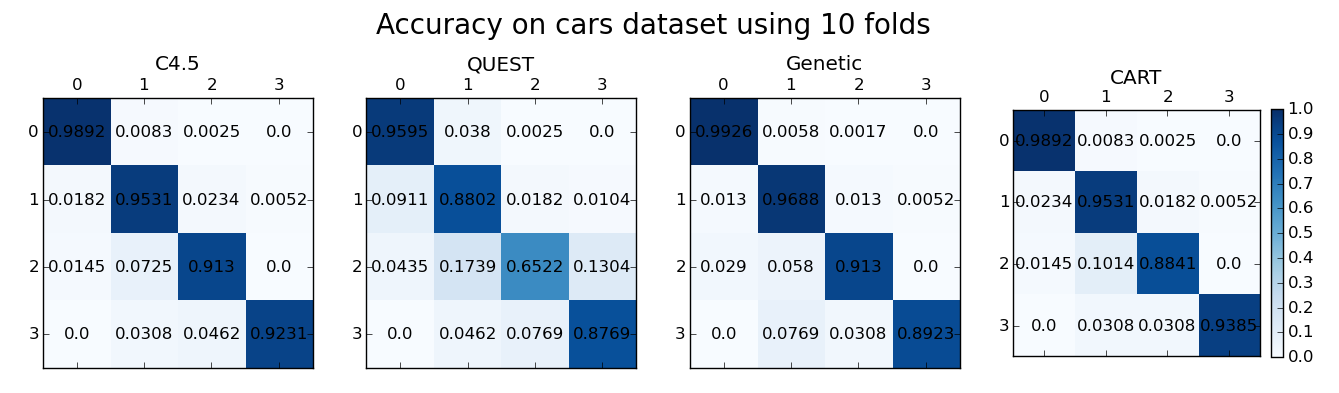
\includegraphics[scale=0.33]{figures/genetic_cars_10_folds.png}
	\end{figure}
\end{frame}

\begin{frame}{Confusion matrix}
	\begin{figure}
		\centering
		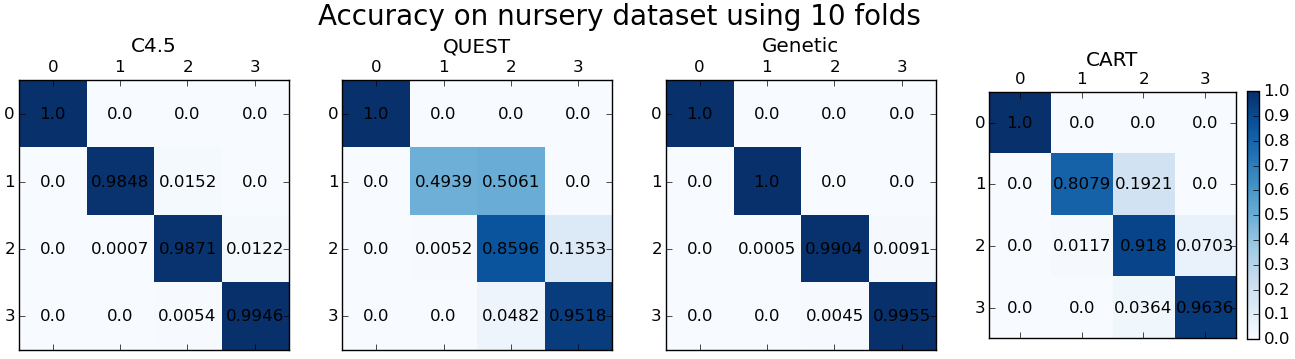
\includegraphics[scale=0.33]{figures/genetic_nurse_10_folds.png}
	\end{figure}
\end{frame}

\section{Visualization}
\section{Conclusion \& future work}




% subsection rstar (end)

% section concensusTeees (end)

\begin{frame}<beamer> 
  \frametitle{Bedankt}
	  {\huge \color{ugentyellow} Bedank voor uw aandacht}\\
	  No written word,
	  
	  No spoken plea,
	  
	  Can teach the youth what they should be,
	  
	  Nor all the books on all the shelves,
	  
	  It's what the teachers are themselves 
\end{frame}

\begin{frame}<beamer> 
	\footnotesize{\tableofcontents[hidesubsections]}
\end{frame}
\end{document}